\documentclass[12pt,letterpaper]{exam}
\usepackage[letterpaper,left=0.5in,right=0.5in,top=0.5in,bottom=0.5in]{geometry}
%\usepackage{toc}

% --- Fonts ---
\usepackage[T1]{fontenc}
\usepackage[utf8]{inputenc}
\usepackage{libertine}

% --- Math ---
\usepackage{amssymb}
\usepackage{amsthm}
\usepackage{mathtools}
\usepackage{bbm}

% --- References ---
\usepackage{hyperref}
\usepackage{cleveref}
\usepackage[style=ieee]{biblatex}       % bibliographies
\addbibresource{/Users/brandonhosley/Documents/GitHub/Schoolwork/Drafts/Mini Prospectus/other/Prospectus.bib}
% --- Other Common Packages ---
%\usepackage{booktabs}
\usepackage{graphicx}
\graphicspath{{../figures/}}
%\usepackage{multicol}
%\usepackage[shortlabels]{enumitem}
%\usepackage[table]{xcolor}
%\usepackage{wrapfig}
%\usepackage{capt-of}
%\usepackage{tikz}
%\usepackage{pgfplots}
%\usetikzlibrary{shapes,arrows,positioning,patterns}
%\usepackage{pythonhighlight}
\usepackage{comment}

%\newcommand\chapter{ X }
\renewcommand{\thequestion}{\textbf{\thesection.\arabic{question}}}
\renewcommand{\questionlabel}{\thequestion}

% -------------------------------- Top Matter -------------------------------- %
\newcommand{\class}{PhD Specialty} % This is the name of the course 
\newcommand{\assignmentname}{Examination} % 
\newcommand{\authorname}{Hosley, Brandon} % 
\newcommand{\workdate}{\today} % 
%\printanswers % this includes the solutions sections

% --------------------------------- Document --------------------------------- %
\begin{document}
\pagestyle{plain}
\thispagestyle{empty}
\noindent
 
% ---------------------------------- Header ---------------------------------- %
\noindent
\begin{tabular*}{\textwidth}{l @{\extracolsep{\fill}} r @{\extracolsep{10pt}} l}
	\textbf{\class} & \textbf{\authorname} &\\%Your name here instead, obviously
	\textbf{\assignmentname } & \textbf{\workdate} & \\
\end{tabular*}\\ 
\rule{\textwidth}{2pt}

% ----------------------------------- Body ----------------------------------- %
\tableofcontents
\hrule


\section{Dr. Yielding's Questions}

While HARL is indeed a subfield of MARL, the distinction between the 
two can often be unclear or inconsistently used in the literature. 
In the broadest sense, 'heterogeneous' may refer to any MARL scenario 
where the agents are not identical. However, using this broad 
definition risks diluting the practical significance of the term.

To provide a more useful distinction, HARL should be invoked when 
the heterogeneity of the agents is fundamental, essential, or definitional 
rather than merely incidental. 
This means the differences among agents are critical to their roles and 
interactions within the system, not just minor variations.

Prior to my literature review, I would have considered HARL to apply 
specifically to cases where agents are distinct from the outset, 
either in their capabilities (For action-space \(\mathcal{A}\), 
\(\mathcal{A}_1 \neq \mathcal{A}_2\)) or their observation spaces
(\(\mathcal{O}_1 \neq \mathcal{O}_2\)). 
This intrinsic heterogeneity is evident in works like \cite{calvo2018} 
(the Irish conference paper mentioned in Dr. Yielding's question)
and implicitly reflected in \cite{berner2019} (OpenAI Five), 
even though they do not explicitly label their methods as HARL.

The most comprehensive source on HARL usage is Zhong et al. \cite{zhong2024}, 
whose work has greatly influenced my understanding. 
They focus on implementing algorithms that encourage the development of 
heterogeneous policies among agents. 
Their framework increases the likelihood of individual agents converging 
on distinct policies, which I term emergent heterogeneity.

In my prospectus, I also mention a suspicion that this approach might not 
entirely prevent agents from converging on policies that are functionally 
similar, thus lacking true diversity. However, this assertion remains an 
ancillary detail as it is not yet substantiated by empirical evidence.

Therefore, I propose distinguishing between intrinsic heterogeneity, where 
agents are fundamentally different before training, and emergent heterogeneity, 
where differences arise as a result of the learning process. 
In the cases where the heterogeneity of the agents falls below a level of 
functional relevance, and appears to be incidental, I argue that they
should not be labeled as HARL. By maintaining these distinctions, 
we can more accurately categorize and understand the applications and 
implications of HARL and MARL.

Below, I apply these distinctions to the cases proposed:

\begin{questions}
	\question
	HAA2C and HADDPG are among the numerous algorithms proposed by 
	Zhong et al.~\cite{zhong2024}. While it seems reasonable that their 
	algorithms could be applied to situations with intrinsic heterogeneity, 
	their implementations and tests are applied to environments with agents 
	that are functionally the same.

	I intend to implement (at least a subset of) their algorithms to the 
	extent that time allows. In doing so, I hope to either corroborate or 
	contradict their results by comparing them to similar algorithms under 
	different conditions. This exploration aims to identify any apparent 
	advantages of these algorithms when applied to the experimental variables 
	proposed for Contribution 1. These experimental variables represent 
	smaller difficulties that we expect to face in Contributions 2 and 3.
	% -------------------------- End Question -------------------------- %

	\question 
	\begin{parts}
		\part
		The scenario described in this part of the question is, perhaps 
		unintuitively, more akin to single-agent than multi-agent reinforcement 
		learning. This becomes clearer when considering a single agent acting 
		as an 'overlord,' where the observation space is a combination of 
		observations from all the individual agents. The actions taken by this 
		overlord are combinations of actions chosen for each agent. 
		Essentially, a single policy processes the combined observation and 
		outputs the combined action.

		\part
		This example is a strong example of MARL, and because the agents
		utilize copies of a singular policy, this example is free from
		any of the types of heterogeneity described in the answer for question
		1.1.

		\part
		The types of problems accurately described by the scenario provided 
		in this part of the question appear to be a subset of MARL problems 
		and a superset of HARL problems.

		Many MARL algorithms allow the member policies to develop distinctly 
		(e.g., \cite{foerster2017, rashid2018, lowe2020}), but they are 
		not optimized to facilitate the development of distinct policies.

		Zhong et al. \cite{zhong2024} formulate their series of HARL 
		algorithms with optimizations intended to facilitate the development 
		of distinct policies. One weakness of this formulation is that there 
		is no guarantee that the multiple policies will not converge to a 
		behaviorally indistinct set, similar to the concept of 
		carcinization observed in evolutionary biology.

		Thus, the resulting heterogeneity of the agents in these scenarios 
		is not intrinsic but emergent. Whether the algorithm itself is 
		labeled as MARL or HARL is distinguished by intent.
	\end{parts}
	% -------------------------- End Question -------------------------- %

	\question
	Referencing Centralized Training Decentralized Execution (CTDE) 
	and Decentralized Training Decentralized Execution (DTDE) as employed 
	by Li et al. in their FA2A paper \cite{li2023d}, we see that CTDE is 
	the most common format for Actor-Critic based MARL algorithms 
	\cite{foerster2017, rashid2018, lowe2020, li2023d, zhou2023}.

	Li et al. \cite{li2023d} and Wen et al. \cite{wen2021} are the only 
	papers I found that discuss the contrary implementation, DTDE. 
	In both cases, the authors motivate DTDE with practical concerns, 
	particularly the limitations of inter-agent communication in 
	distributed systems. These considerations are important, but the 
	relation to HARL remains the same as described in answer 1.2 (c).
	% -------------------------- End Question -------------------------- %
\end{questions}




%%%%%%%%%%%%%%%%%%%%%%%%%%%%%%%%%%%%%%%%%%%%%%%%%%%%%%%%%%%%%%%%%%%%%%%%%%%%%%%%
% --------------------------------- Edit Bar --------------------------------- %
%%%%%%%%%%%%%%%%%%%%%%%%%%%%%%%%%%%%%%%%%%%%%%%%%%%%%%%%%%%%%%%%%%%%%%%%%%%%%%%%



\section{Dr. Robbins' Questions}



\begin{figure}[h]
	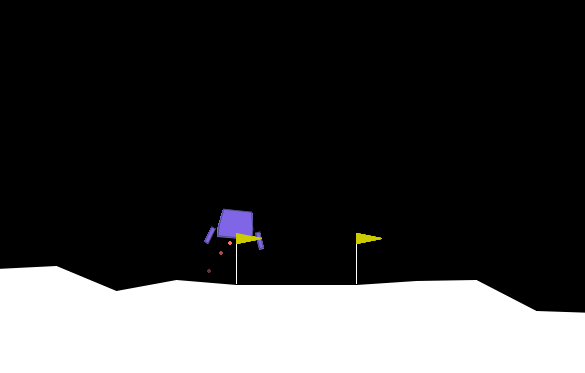
\includegraphics[width=.3\linewidth]{single_lander.png}
	\caption{Lunar Lander}
\end{figure}



\section{Dr. Cox's Questions}

\end{document}
